\subsection{Signalanalyse}
\label{sec:Signalanalyse}
\subsubsection{Anschlagserkennung}
Zur Erkennung von Anschlägen und Abgrenzung von Hintergrundrauschen werden die Messdaten in Echtzeit geprüft. 
Hierzu werden die jeweils letzten beiden Messwerte miteinander verglichen. 
Ein Anschlag wird erkannt, wenn der aktuellere Wert den vorherigen Wert um ein bestimmtes Vielfaches der Standartabweichung übersteigt. 
Der Faktor sollte dabei auf das zu erwartende Rauschen abgestimmt werden.
Höhere Werte neigen weniger dazu, Ausschläge im Rauschen bzw. unabsichtliche Berührungen der Oberfläche als Anschlag zu erkennen.
Niedrigere Werte erlauben dagegen, auch sanfte Anschläge zu erkennen.
In unseren Versuchen hat sich ein Faktor von sechs als stabil erwiesen.

Wurde ein Anschlag erkannt, so beginnt ein Zeitfenster von ca. 500ms, in dem eingehende Messwerte gepuffert werden. 
Nach Ablauf des Zeitfensters wird dem Programm signalisiert, dass ein Schlag aufgenommen wurde. 
Zusätzlich werden die Messwerte bis ca. 20ms vor dem erkannten Anschlag in die Zeitreihe aufgenommen.

\subsubsection{Analyse der Beschleunigungsdaten}
\label{sec:Analyse-a}
Die Klassifizierung aufgenommener Schläge erfolgt mittels Auswertung der stärksten Frequenzen. 
Hierzu werden die Messwerte zunächst einer diskreten Fouriertransformation unterzogen, und die Spektrale Leistungssdichte der Zeitreihe bestimmt.
In der aktuellen Implementierung konnten Abtastraten von ca. 200Hz erreicht werden. 
Die größte detektierbare Frequenz $f_{max}$ liegt somit bei 100Hz.

Für ein Zeitfenster von ca. 500ms ergeben sich 128 Messwerte.
Nach Anwendung der Fouriertransformation erhält man somit 64 diskrete Frequenzgruppen mit einer Trennschärfe von ca. 2Hz.

Aus diesen Daten werden die vier Frequenzgruppen mit der höchsten Amplitude ermittelt und zur weiteren Verwendung gespeichert.

Um verschiedene Oberflächen auf ihre Eignung zu untersuchen, erweiterten wir unsere App um eine Funktion zur Darstellung der FFT-Analyse. Abbildung \ref{fig:guiA} zeigt die Analyse einer aufgenommenen Schwingung in einem frühen Stadium des Projektes.

\begin{figure}[H]Lernphase
	\centering
	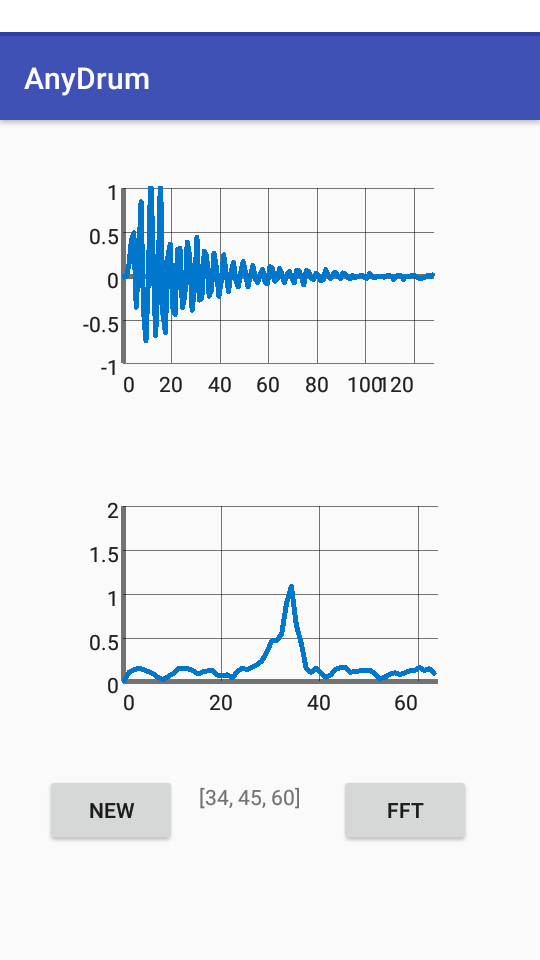
\includegraphics[scale=0.4]{figures/gui_FFT.png}
	\caption{Analyse eines aufgenommenen Schlages mit FFT-Analyse und größten Maxima. Die Abbildung entstand mit einer frühen Version der Android-App, die noch den Beschleunigungssensor des Smartphones verwendete. Aufgrund der niedrigen Samplerate ist die Schwingung bereits nach 80 Messwerten abgeklungen. Weiterhin wurden zu diesem Zeitpunkt nur die drei stärksten Maxima ermittelt.}
	\label{fig:guiA}
\end{figure}


\subsubsection{Lernphase}
\label{sec:Lernphase}
Zum Erlernen einer Schlagposition werden zwölf Schläge aufgezeichnet und wie oben in Abschnitt \ref{sec:Analyse-a} beschrieben analysiert.
Anschließend wird der Durchschnitt der jeweils stärksten Frequenzgruppe, zweitstärksten Frequenzgruppe, usw. ermittelt, wie in Abb. \ref{fig:FFT_Mittelwerte} zu sehen ist. 
Diese werden als charakteristisches Muster gespeichert.

Tabelle \ref{tab:FFT} zeigt die zwölf Schläge zum Lernen für Hihat und Bass.
Die Schläge wurden auf einer Tischplatte ausgeführt mit unterschiedlicher Position für HiHat und Bass.

Es ist zu erkennen, dass die Unterschiede zwischen den Arithm. Mittelwerten deutlich größer sind, als zwischen den Median-Werte in Abb. \ref{fig:FFT_Median}. 
Aufgrund dieser Beobachtung wurde das Arithm. Mittel gewählt, um das charakteristische Muster zu erzeugen. 
Weiterhin ist erkennbar, das die Unterschiede selbst bei der viertstärksten Frequenzgruppe noch deutlich sind.
Wurden zusätzlich die fünftstärksten, sechststärksten, etc. Frequenzgruppen mit einbezogen, verloren diese zunehmend an Signifikanz und das Ergebnis der Klassifikation wurde ungenauer.


\begin{table}[H]
	\centering
	\caption{Stärkste Frequenzgruppen aus jeweils zwölf Schlägen für HiHat und Bass}
	\begin{tabular}{l c c c c | l c c c c}
		HiHat &&&& &Bass \\
		\hline
		Frequenzgruppe & $F_1$ & $F_2$ & $F_3$ & $F_4$  & & $F_1$ & $F_2$ & $F_3$ & $F_4$\\	
		
        & 6	 & 13  & 8  & 18 && 6  & 52 &	58 & 41\\
        & 15 &	19 & 7  & 10 && 6  & 14 &	18 & 10\\
        & 5  &	24 & 15	& 11 && 17 & 23 &	11 & 29\\
        & 14 &	18 & 7  & 26 && 6  & 27 &	11 & 31\\
        & 8	 &  16 & 12 & 23 && 7  & 11 &	21 & 15\\
        & 5  &	12 & 16 & 21 && 6  & 27 &	15 & 10\\
        & 14 &	7  & 20	& 4  && 10 & 45 &	60 & 21\\
        & 8	 &  30 & 41 & 14 &&  6 & 10 &	15 & 27\\
        & 21 &	24 & 31 & 7  &&  9 & 10 &	14 & 30\\
        & 12 &	18 & 23 & 35 &&  9 & 11 &	5  & 18\\
        & 11 &	23 &  6 & 18 &&  7 & 14 &	31 & 20\\
        & 17 &	11 &  7 &  4 &&  6 & 29 &	36 & 58\\
        		\\
		\hline
		Arithm. Mittel & 11.3 & 17.9 & 16.1 &	15.9  && 7.9 & 22.8 &	24.6 &	25.8\\
		Median       & 11.5 & 18   & 13.5 &	16    && 6.5 & 18.5 &	16.5 &	24\\		 

 
        
%        & 13 & 14 & 15 & 19  &&13& 114& 115& 87\\
%		& 30 & 31 & 23 & 24 &&13& 28& 29& 30\\
%		& 13& 14& 15& 16 &&35& 36& 23& 24\\
%		& 29& 30& 13&36 &&13& 14& 15& 62\\
%		& 17& 23&24& 30 	&&15& 16& 42& 43\\
%		&13& 24& 25& 47	&&13& 54& 30& 31\\
%
%		&27& 15& 16& 17	&&20& 89& 90& 39\\
%
%		 &17& 18& 30& 31 &&13& 20& 26& 27\\
%
%		&42& 43& 44& 55		&&19& 20& 29& 30\\
%
%		 &25& 33& 34& 35 &&19& 20& 13& 26 \\
%
%		&22& 23& 13& 37		&&13& 14& 15& 16\\
%
%		&31& 32& 14& 15  &&13& 58& 59& 60\\
%		\\
%		\hline
%		Durchschnitt & 23,25&	25	&22,167& 30,167 && 16,583	&40,25&	40,5&	39,583	\\
%		Median & 23,5 &	23,5& 19,5	& 30,5 && 13 &	24	& 29	 &30,5 \\		 
		

	\end{tabular}
	\label{tab:FFT}
\end{table}

\begin{figure}[H]
\centering
\begin{subfigure}{.5\textwidth}
		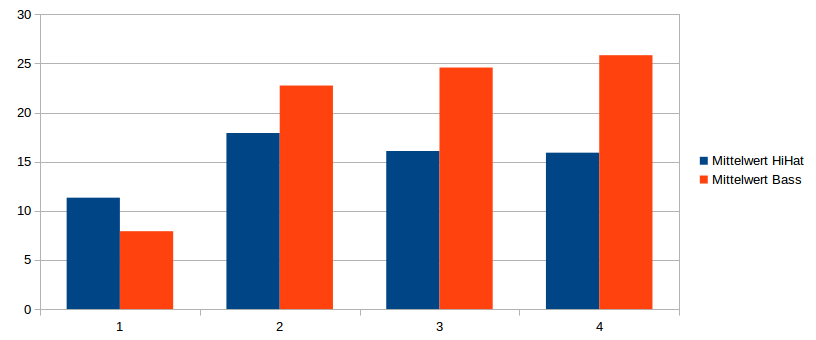
\includegraphics[scale=0.5]{figures/Mittelwert_2.png}
\end{subfigure}
\caption{Arithm. Mittel von Hihat und Bass für Frequenzen F1 - F4}
\label{fig:FFT_Mittelwerte}
\end{figure}


\begin{figure}[H]
\centering
\begin{subfigure}{.5\textwidth}
		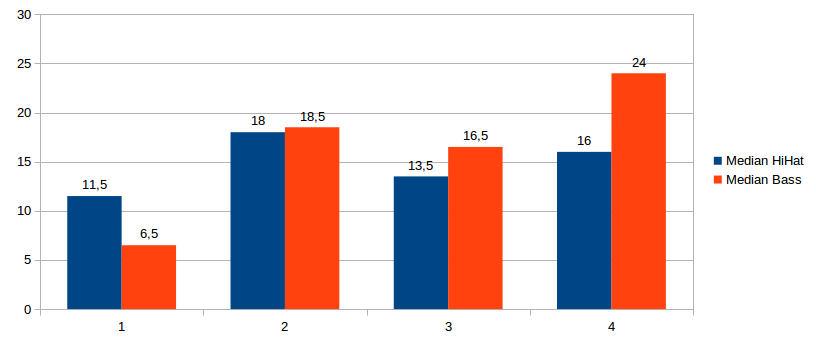
\includegraphics[scale=0.5]{figures/Median_2.png}
\end{subfigure}
\caption{Median von Hihat und Bass für Frequenzen F1 - F4}
\label{fig:FFT_Median}
\end{figure}


\subsubsection{Echtzeit-Klassifizierung}
Ist die Echtzeit-Klassifizierung aktiviert, so werden nach erfolgter Anschlagserkennung und Schlagaufzeichnung die Messwerte analysiert und mit denen der gelernten Positionen verglichen. 
Für diesen Vergleich werden die Frequenzabstände der jeweils stärkste Frequenzgruppen, zweitstärksten Frequenzgruppen, usw. ermittelt und die Teilergebnisse zu einer totalen Abweichung aufsummiert.

Nachfolgend ist so eine Klassifizierung mittels der im Abschnitt \ref{sec:Lernphase} eingeführten Beispieldaten dargestellt.
Nach erfolgter Lernphase wurde ein Anschlag aufgenommen und analysiert:

Dominateste Frequenzgruppen des Anschlages: 
\begin{tabular}{c c c c}
$F_1$ & $F_2$ & $F_3$ & $F_4$\\
\hline
 13  &	18 &	7 &	28\\
\end{tabular}

Berechnung der Frequenzabstände:
\begin{displaymath}
Error_{position} = \sum_{i=1}^{4} \lvert F_{i,schlag} - F_{i,position}\rvert
\end{displaymath}

ergibt folgende Fehlerwerte:


\begin{align*}
Error_{HiHat} &= \sum_{i=1}^{4}  \lvert F_{i,schlag} - F_{i,HiHat}\rvert \\
Error_{HiHat} &= \lvert(13-11.3)\rvert + \lvert(18-17.9)\rvert + \lvert(7-16.1)\rvert + \lvert(28-15.9)\rvert \\
Error_{HiHat} &= 23
\end{align*}


\begin{align*}
Error_{Base} &= \sum_{i=1}^{4} \lvert F_{i,schlag} - F_{i,Base}\rvert \\
Error_{Base} &= \lvert (13-7.9)\rvert + \lvert(18-22.8)\rvert + \lvert(7-24.6)\rvert + \lvert(28-25.8)\rvert \\
Error_{Base} &= 30,7
\end{align*}

Der Fehlerwert für HiHat ist geringer.
Demzufolge wird die angeschlagene Position als HiHat-Position klassifiziert.
 
Erkennbar hierbei ist, dass in jedem Falle eine Zuordnung erfolgt, auch wenn die Abweichung sehr groß ist. 
Dies könnte jedoch leicht geändert werden, indem eine maximale Abweichung festgelegt wird und alle berechneten Abweichungen, die diesen Wert übersteigen, als nicht klassifizierbar eingestuft werden. 
Alternativ könnte, ähnlich zu anderen Clustering-Verfahren, eine Nachbarschaftsbeziehung zur Klassifikation verwendet werden.

\subsubsection{Signalaufbereitung und Filterung}

In der aktuellen Implementierung wird keine Filterung der Messdaten vorgenommen. 
Um die Genauigkeit der Frequenzanalyse zu erhöhen, sollten die Messwerte vor Anwendung der FFT mit einem Tiefpassfilter mit der Grenzfrequenz $f_{max}$ gefiltert werden.

Eine Möglichkeit, um Rauschen zu unterdrücken wäre die Nutzung eines Grenzwertes. Auf diese Art können schwache Erschütterungen und leichte Vibrationen unterdrückt werden.
Die Sensordaten könnten weiter geglättet werden durch Verwendung eines Box-Filters (Moving-Average) oder Gauss-Filters.

%Anstelle von timbreID, welches laut Entwickler \cite{timbreID} Cluster benutzt und Merkmale sortiert, haben wir den DBSCAN-Algorithmus getetest.

%Elbatta und Ashour untersuchen verschiedene Clustering Ansätze und stellen in ihrer Arbeit \cite{Elbatta2013ADM} einen verbesserten DBSCAN-Algorithmus vor.
%DBSCAN ist ein  dichtebasierter Cluster-Algorithmus, der als Parameter einen Radius und eine Mindestanzahl an Punkte pro Cluster benötigt.
%Im Gegensatz zu partitionierungsbasierten Cluster-Algorithmen, wie zum Beispiel K-Means, besitzt DBSCAN dne Vorteil, dass es freie Formen von Clustern erkennen kann und sich besonders gut für Daten mit %Rauschen eignet.
%Der Algorithmus startet mit einem zufälligen Punkt.
%Befinden sich die Mindestanzahl an Nachbarpunkten um den gewählten Punkt im gegebenen Radius, wird ein Cluster mit allen gefunden Punkten gebildet.
%Ist die Anzahl Nachbarpunkte kleiner als die Mindestanzahl wird dies als Rauschen markiert.
%Es wird rekursiv mit dem nächsten freien Punkt verfahren, der noch nicht zu einem Cluster gehört und noch nicht bewertet wurde.

%Der DBSCAN-Algorithmus könnte somit verwendet werden, um besondere Merkmale von festzustellen und diese von Rauschen zu unterscheiden.

%Ein Clustering mit DBSCAN zeigte bei uns keine guten Ergebnisse, da wohl die Merkmale
